%======================================================================
\section{Results}\label{sec:results}
%======================================================================
\subsection{Peak and bill reduction}
Tables~\ref{tab:main} and~\ref{tab:service} report six-month means with the range of monthly values, including the split of each bill into energy and demand charges. The demand charge is 69\% of the uncontrolled bill at both sites. At JPL uncontrolled charging exceeds the 195\,kW capacity (mean monthly peak 296\,kW), and EDF and LLF cut the bill by 23\% only by capping the peak at that limit; at Caltech the uncontrolled peak (105\,kW) never reaches the 150\,kW capacity, so EDF and LLF coincide with uncontrolled charging.

Nominal MPC reduces the mean monthly site peak from 296 to 140\,kW at JPL ($-53\%$) and from 105 to 52\,kW at Caltech ($-50\%$), a reduction of 156\,kW and 53\,kW of peak demand at the grid connection (monthly values in Fig.~S2). The mean monthly bill falls from 6,693 to 4,234\,USD at JPL ($-37\%$) and from 2,355 to 1,537\,USD at Caltech ($-35\%$). The weekday load profiles in Fig.~\ref{fig:profiles} show the mechanism: the controller flattens the morning arrival spike into a plateau and shifts energy away from the 12--18\,h summer on-peak window. The hindsight optimum shows how much is achievable with full information. With every session fully served it costs 3,913\,USD at JPL and 1,291\,USD at Caltech, with mean peaks of 110\,kW and 35\,kW.

\begin{table}[!htbp]
\centering
\caption{Monthly electricity cost by policy (July--December 2019).}
\label{tab:main}
\footnotesize
\setlength{\tabcolsep}{1.5pt}
\begin{tabular*}{\textwidth}{@{\extracolsep{\fill}}llrrrrr@{}}
\hline
Site & Policy & \makecell[c]{Bill\\(USD)} & \makecell[c]{Energy\\(USD)} & \makecell[c]{Demand\\(USD)} & \makecell[c]{Gap to\\opt. (\%)} & \makecell[c]{Penalised\\(USD)} \\
\hline
JPL & Uncontrolled & 6,693\,{\scriptsize(6,085--7,500)} & 2,103 & 4,589 & +74.0 & 6,693 \\
JPL & EDF & 5,171\,{\scriptsize(4,532--5,755)} & 2,146 & 3,024 & +33.7 & 5,289 \\
JPL & LLF & 5,147\,{\scriptsize(4,530--5,705)} & 2,123 & 3,024 & +33.2 & 5,156 \\
JPL & Nominal MPC & 4,234\,{\scriptsize(3,542--4,938)} & 2,066 & 2,168 & +8.9 & 8,468 \\
JPL & Robust MPC, $q$=0.5 & 3,079\,{\scriptsize(2,487--3,653)} & 1,763 & 1,317 & -21.1 & 27,951 \\
JPL & Robust MPC, $q$=0.7 & 3,705\,{\scriptsize(3,119--4,268)} & 1,975 & 1,730 & -4.7 & 15,625 \\
JPL & Robust MPC, $q$=0.9 & 4,586\,{\scriptsize(4,012--5,176)} & 2,052 & 2,534 & +18.6 & 8,531 \\
JPL & MPC + top-up & 4,376\,{\scriptsize(3,609--5,150)} & 2,208 & 2,168 & +12.4 & 4,610 \\
JPL & MPC + top-up, $q$=0.7 & 4,085\,{\scriptsize(3,290--4,876)} & 2,354 & 1,730 & +4.3 & 5,762 \\
JPL & MPC + top-up, $q$=0.9 & 4,681\,{\scriptsize(4,079--5,325)} & 2,157 & 2,524 & +20.9 & 4,754 \\
JPL & Hindsight opt. & 3,913\,{\scriptsize(3,086--4,682)} & 2,212 & 1,701 & +0.0 & 3,913 \\
\hline
Caltech & Uncontrolled & 2,355\,{\scriptsize(1,949--2,697)} & 729 & 1,627 & +86.3 & 2,355 \\
Caltech & EDF & 2,355\,{\scriptsize(1,949--2,697)} & 729 & 1,627 & +86.3 & 2,355 \\
Caltech & LLF & 2,355\,{\scriptsize(1,949--2,697)} & 729 & 1,627 & +86.3 & 2,355 \\
Caltech & Nominal MPC & 1,537\,{\scriptsize(1,092--1,795)} & 731 & 806 & +19.5 & 2,849 \\
Caltech & Robust MPC, $q$=0.5 & 1,000\,{\scriptsize(678--1,193)} & 550 & 450 & -22.6 & 10,883 \\
Caltech & Robust MPC, $q$=0.7 & 1,315\,{\scriptsize(954--1,628)} & 678 & 637 & +2.1 & 5,595 \\
Caltech & Robust MPC, $q$=0.9 & 1,515\,{\scriptsize(1,041--1,849)} & 716 & 799 & +17.3 & 3,731 \\
Caltech & MPC + top-up & 1,576\,{\scriptsize(1,102--1,869)} & 770 & 806 & +22.3 & 1,837 \\
Caltech & MPC + top-up, $q$=0.7 & 1,423\,{\scriptsize(989--1,814)} & 786 & 637 & +10.0 & 2,436 \\
Caltech & MPC + top-up, $q$=0.9 & 1,556\,{\scriptsize(1,063--1,895)} & 763 & 793 & +20.4 & 1,962 \\
Caltech & Hindsight opt. & 1,291\,{\scriptsize(895--1,607)} & 750 & 541 & +0.0 & 1,291 \\
\hline
\end{tabular*}
\par\smallskip\parbox{\textwidth}{\scriptsize Six-month means; the range of monthly values is shown in parentheses. Gap is the mean monthly bill gap to the hindsight optimum; Penalised adds 5\,USD per undelivered kWh.}
\end{table}


\begin{table}[!htbp]
\centering
\caption{Monthly peak demand and charging service by policy (July--December 2019).}
\label{tab:service}
\footnotesize
\setlength{\tabcolsep}{1.5pt}
\begin{tabular*}{\textwidth}{@{\extracolsep{\fill}}llrrr@{}}
\hline
Site & Policy & \makecell[c]{Peak\\(kW)} & \makecell[c]{Energy served\\(\%)} & \makecell[c]{EVs fully\\served (\%)} \\
\hline
JPL & Uncontrolled & 296\,{\scriptsize(284--313)} & 100.0\,{\scriptsize(100.0--100.0)} & 100.0\,{\scriptsize(100.0--100.0)} \\
JPL & EDF & 195\,{\scriptsize(195--195)} & 99.9\,{\scriptsize(99.9--99.9)} & 99.5\,{\scriptsize(99.3--99.7)} \\
JPL & LLF & 195\,{\scriptsize(195--195)} & 100.0\,{\scriptsize(100.0--100.0)} & 99.9\,{\scriptsize(99.8--100.0)} \\
JPL & Nominal MPC & 140\,{\scriptsize(128--154)} & 96.0\,{\scriptsize(94.9--97.3)} & 86.6\,{\scriptsize(84.1--89.1)} \\
JPL & Robust MPC, $q$=0.5 & 85\,{\scriptsize(78--91)} & 76.8\,{\scriptsize(75.3--78.1)} & 40.0\,{\scriptsize(37.7--43.3)} \\
JPL & Robust MPC, $q$=0.7 & 112\,{\scriptsize(103--116)} & 88.8\,{\scriptsize(87.9--90.6)} & 62.8\,{\scriptsize(60.1--65.2)} \\
JPL & Robust MPC, $q$=0.9 & 163\,{\scriptsize(151--173)} & 96.3\,{\scriptsize(95.4--97.3)} & 84.7\,{\scriptsize(81.0--87.0)} \\
JPL & MPC + top-up & 140\,{\scriptsize(128--154)} & 99.8\,{\scriptsize(99.7--99.9)} & 98.9\,{\scriptsize(98.5--99.7)} \\
JPL & MPC + top-up, $q$=0.7 & 112\,{\scriptsize(103--116)} & 98.4\,{\scriptsize(98.0--99.0)} & 94.0\,{\scriptsize(92.9--96.1)} \\
JPL & MPC + top-up, $q$=0.9 & 163\,{\scriptsize(150--173)} & 99.9\,{\scriptsize(99.8--100.0)} & 99.6\,{\scriptsize(99.1--99.9)} \\
JPL & Hindsight opt. & 110\,{\scriptsize(98--124)} & 100.0\,{\scriptsize(100.0--100.0)} & 100.0\,{\scriptsize(100.0--100.0)} \\
\hline
Caltech & Uncontrolled & 105\,{\scriptsize(89--121)} & 100.0\,{\scriptsize(100.0--100.0)} & 100.0\,{\scriptsize(100.0--100.0)} \\
Caltech & EDF & 105\,{\scriptsize(89--121)} & 100.0\,{\scriptsize(100.0--100.0)} & 100.0\,{\scriptsize(100.0--100.0)} \\
Caltech & LLF & 105\,{\scriptsize(89--121)} & 100.0\,{\scriptsize(100.0--100.0)} & 100.0\,{\scriptsize(100.0--100.0)} \\
Caltech & Nominal MPC & 52\,{\scriptsize(44--57)} & 96.3\,{\scriptsize(94.8--97.2)} & 87.6\,{\scriptsize(84.4--89.7)} \\
Caltech & Robust MPC, $q$=0.5 & 29\,{\scriptsize(24--33)} & 71.7\,{\scriptsize(69.3--76.0)} & 44.9\,{\scriptsize(40.6--49.6)} \\
Caltech & Robust MPC, $q$=0.7 & 41\,{\scriptsize(37--46)} & 87.9\,{\scriptsize(85.8--89.5)} & 65.3\,{\scriptsize(63.3--67.9)} \\
Caltech & Robust MPC, $q$=0.9 & 51\,{\scriptsize(42--55)} & 93.6\,{\scriptsize(91.8--95.5)} & 80.1\,{\scriptsize(77.8--82.2)} \\
Caltech & MPC + top-up & 52\,{\scriptsize(44--57)} & 99.2\,{\scriptsize(99.0--99.6)} & 96.0\,{\scriptsize(94.5--97.3)} \\
Caltech & MPC + top-up, $q$=0.7 & 41\,{\scriptsize(37--46)} & 97.1\,{\scriptsize(96.5--97.9)} & 90.5\,{\scriptsize(89.5--92.6)} \\
Caltech & MPC + top-up, $q$=0.9 & 51\,{\scriptsize(42--55)} & 98.8\,{\scriptsize(97.0--99.4)} & 95.9\,{\scriptsize(91.9--97.5)} \\
Caltech & Hindsight opt. & 35\,{\scriptsize(30--40)} & 100.0\,{\scriptsize(100.0--100.0)} & 100.0\,{\scriptsize(100.0--100.0)} \\
\hline
\end{tabular*}
\par\smallskip\parbox{\textwidth}{\scriptsize Six-month means with the range of monthly values in parentheses. A vehicle is fully served when its shortfall is at most 0.05\,kWh.}
\end{table}






\begin{figure}[!htbp]
\centering
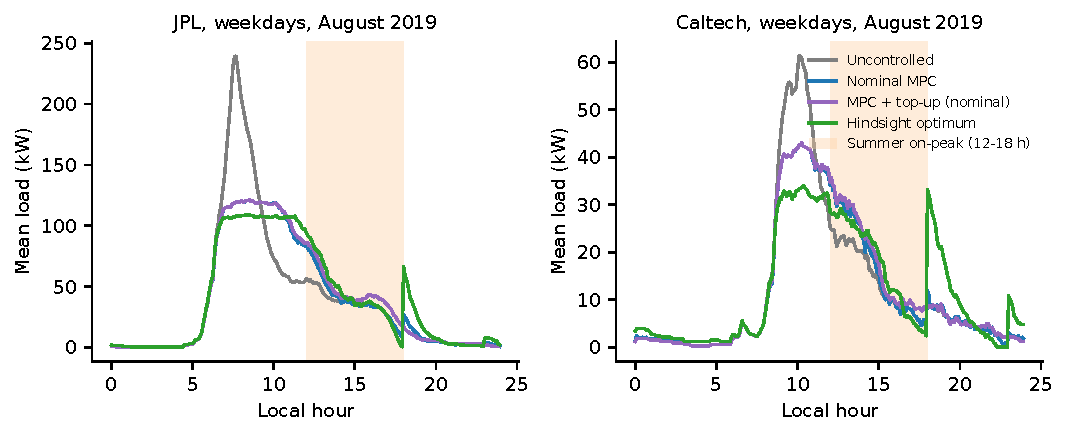
\includegraphics[width=0.7\textwidth]{figures/Fig4_load_profiles.pdf}
\caption{Mean weekday load profiles in August 2019. The shaded band is the TOU-EV-4 summer on-peak period.}
\label{fig:profiles}
\end{figure}

\subsection{Realised grid flexibility}\label{sec:res:flex}
Table~\ref{tab:flex} reports the grid-flexibility metrics of Section~\ref{sec:metrics}; normalised load-duration curves are shown in Fig.~S3 of the Supplementary Material.
\emph{Uncontrolled load is extremely peaky.} Its peak-to-average ratio is 10.2 (JPL) and 11.2 (Caltech): the site connection is sized for a load that occurs for a few hours on weekday mornings. \emph{Peak-state control roughly halves that ratio.} PAR falls to 4.8--5.0 (JPL) and 5.6--5.8 (Caltech), the load factor doubles, and the steepest 15-min ramp falls by 31\% (JPL) and 20\% (Caltech). This is achieved by moving 14--17\% (JPL) and 9--14\% (Caltech) of the monthly energy away from the time uncontrolled charging would have drawn it. \emph{Top-up does not erode the flexibility gain.} It leaves the peak unchanged and only raises the load factor further, because it fills existing headroom. \emph{Combining moderate robustness with top-up delivers most of the achievable flexibility.} At $q=0.7$ the peak reduction reaches 62\% (JPL) and 61\% (Caltech), close to the hindsight optimum (63\% and 67\%). The online controller also avoids the large ramps that the hindsight schedule produces at tariff-period boundaries at JPL (99\,kW per 15\,min, against 43\,kW). \emph{LLF delivers peak reduction only through the capacity cap.} It cuts the JPL peak by 34\% exactly to the 195\,kW limit and does nothing at Caltech, where capacity does not bind.
\begin{table}[!htbp]
\centering
\caption{Grid-flexibility metrics (July--December 2019).}
\label{tab:flex}
\footnotesize
\setlength{\tabcolsep}{1.5pt}
\begin{tabular*}{\textwidth}{@{\extracolsep{\fill}}llrrrrr@{}}
\hline
Site & Policy & \makecell[c]{Peak\\red. (\%)} & \makecell[c]{Load\\factor} & PAR & \makecell[c]{Max ramp\\(kW/15 min)} & \makecell[c]{Shifted\\(\%)} \\
\hline
JPL & Uncontrolled & 0.0\,{\scriptsize(0.0--0.0)} & 0.099 & 10.2\,{\scriptsize(8.8--10.8)} & 73.1 & 0.0 \\
JPL & LLF & 34.0\,{\scriptsize(31.3--37.7)} & 0.149 & 6.7\,{\scriptsize(5.9--7.1)} & 59.2 & 4.3 \\
JPL & Nominal MPC & 52.7\,{\scriptsize(45.6--56.1)} & 0.201 & 5.0\,{\scriptsize(4.0--5.6)} & 50.3 & 17.3 \\
JPL & Robust MPC, $q$=0.9 & 44.7\,{\scriptsize(40.8--51.5)} & 0.173 & 5.9\,{\scriptsize(4.7--6.5)} & 55.0 & 15.3 \\
JPL & MPC + top-up & 52.7\,{\scriptsize(45.6--56.1)} & 0.209 & 4.8\,{\scriptsize(3.9--5.4)} & 49.7 & 13.8 \\
JPL & MPC + top-up, $q$=0.7 & 62.3\,{\scriptsize(59.1--64.9)} & 0.258 & 3.9\,{\scriptsize(3.2--4.2)} & 42.9 & 20.1 \\
JPL & Hindsight opt. & 62.9\,{\scriptsize(56.2--67.6)} & 0.268 & 3.8\,{\scriptsize(3.0--4.3)} & 98.8 & 21.9 \\
\hline
Caltech & Uncontrolled & 0.0\,{\scriptsize(0.0--0.0)} & 0.091 & 11.2\,{\scriptsize(9.8--13.5)} & 34.3 & 0.0 \\
Caltech & LLF & 0.0\,{\scriptsize(0.0--0.0)} & 0.091 & 11.2\,{\scriptsize(9.8--13.5)} & 34.3 & 0.0 \\
Caltech & Nominal MPC & 49.9\,{\scriptsize(35.4--55.3)} & 0.176 & 5.8\,{\scriptsize(5.0--6.7)} & 27.4 & 13.7 \\
Caltech & Robust MPC, $q$=0.9 & 50.5\,{\scriptsize(42.0--58.0)} & 0.172 & 5.8\,{\scriptsize(5.3--6.3)} & 28.2 & 18.9 \\
Caltech & MPC + top-up & 49.9\,{\scriptsize(35.4--55.3)} & 0.181 & 5.6\,{\scriptsize(4.8--6.5)} & 27.2 & 9.3 \\
Caltech & MPC + top-up, $q$=0.7 & 60.6\,{\scriptsize(54.3--65.8)} & 0.224 & 4.5\,{\scriptsize(3.7--5.3)} & 23.4 & 15.8 \\
Caltech & Hindsight opt. & 66.7\,{\scriptsize(61.9--69.2)} & 0.272 & 3.7\,{\scriptsize(3.2--4.2)} & 34.9 & 22.1 \\
\hline
\end{tabular*}
\par\smallskip\parbox{\textwidth}{\scriptsize Means with monthly ranges in parentheses. Peak reduction and shifted energy are relative to uncontrolled charging; PAR is the peak-to-average ratio of the monthly load.}
\end{table}




\subsection{Coincidence with on-site solar}\label{sec:res:pv}
Flattening the morning spike moves charging towards midday, although the controllers receive no PV signal. With an energy-neutral clear-sky PV array, the share of EV energy coincident with PV rises from 46.7\% under uncontrolled charging to 53.4\% with MPC + top-up and 60.5\% at $q=0.7$ at JPL, and from 56.1\% to 59.7\% and 64.3\% at Caltech (Table~S3 and Fig.~S4 of the Supplementary Material; with a half-size array the gains have the same sign). The same shift has a cost under this tariff: the share of energy in the 12--18\,h on-peak block rises from 24.7\% to 28.3\% (JPL) and from 26.9\% to 33.9\% (Caltech), and the energy cost rises by about 5\%. The demand-charge and energy-price signals pull in opposite directions, and the demand charge wins because it is 69\% of the uncontrolled bill. Section~\ref{sec:res:pvaware} tests a PV-aware objective and Section~\ref{sec:res:arch} tariffs that remove this conflict.

\subsection{The service cost of acting on declarations}\label{sec:res:diag}
The bill reduction of nominal MPC is not free. It serves 96.0\% (JPL) and 96.3\% (Caltech) of the demanded energy, and only 86.6\% and 87.6\% of vehicles leave with their full energy. The hindsight optimum serves every vehicle at a lower bill, so the shortfall is caused by missing information, not by the tariff or the capacity limit. Valued at the base penalty of 5\,USD/kWh, the penalised cost of nominal MPC (8,468\,USD at JPL, 2,849\,USD at Caltech) is higher than that of LLF at JPL and of uncontrolled charging at Caltech.

Fig.~\ref{fig:unmet} decomposes the undelivered energy into its two causes. The first is vehicles whose declared energy was delivered but was below what they actually accepted: 45\% of the 5,080\,kWh left undelivered at JPL over the six months, and 31\% of 1,575\,kWh at Caltech. The second is vehicles that departed before their declared energy had been delivered (the remaining 55\% and 69\%). Both causes follow from the declaration errors in Fig.~\ref{fig:errors}. Most drivers over-request energy, but a minority under-request, and about a third leave earlier than declared.

\begin{figure}[!htbp]
\centering
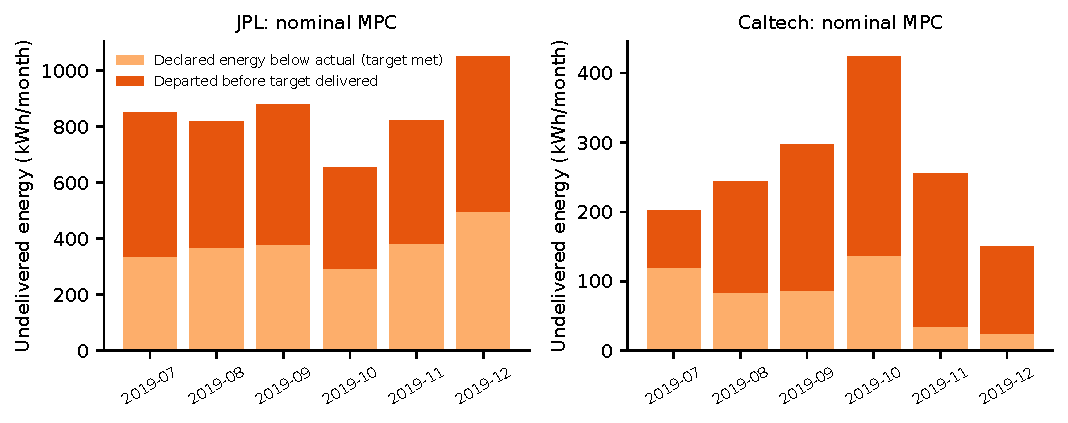
\includegraphics[width=0.7\textwidth]{figures/Fig10_unmet_decomposition.pdf}
\caption{Undelivered energy of nominal MPC by cause: declared energy below the energy actually accepted (target met), and departure before the declared energy was delivered.}
\label{fig:unmet}
\end{figure}

\subsection{Calibrated robustness does not close the gap}\label{sec:res:robust}
The calibrated sets are shown in Fig.~S5 of the Supplementary Material. At $q=0.5$ the controller moves deadlines 0.5--1\,h later and scales declared energy down to 0.52--0.65 of its declared value, because the median driver stays longer and receives less than declared. At $q=0.9$ deadlines move 1.3--2.8\,h earlier while the energy multiplier only returns to about 1.0. The upward bias of declared energy is so strong that even the 90th percentile of $\rho$ does not exceed one for claimed sessions.



The consequences are shown in Fig.~\ref{fig:frontier}. Robust MPC at $q=0.5$ and $0.7$ produces the lowest bills in the study, below the hindsight optimum at JPL for both levels and at Caltech for $q=0.5$. It does so by delivering only 72--89\% of the energy, so the saving is a service cut rather than better scheduling. At $q=0.9$ the energy served returns to the nominal level at JPL (96.3\%) but the earlier deadlines raise the peak to 163\,kW, increasing the bill by 8\% over nominal MPC. At Caltech, energy served at $q=0.9$ (93.6\%) remains below nominal. No protection level improves on nominal MPC in penalised cost at either site. The quantile box can shift and scale targets, but it cannot create energy targets for the minority of vehicles whose needs exceed their declarations, and protecting early leavers requires deadlines so early that the peak rises.

\begin{figure}[!htbp]
\centering
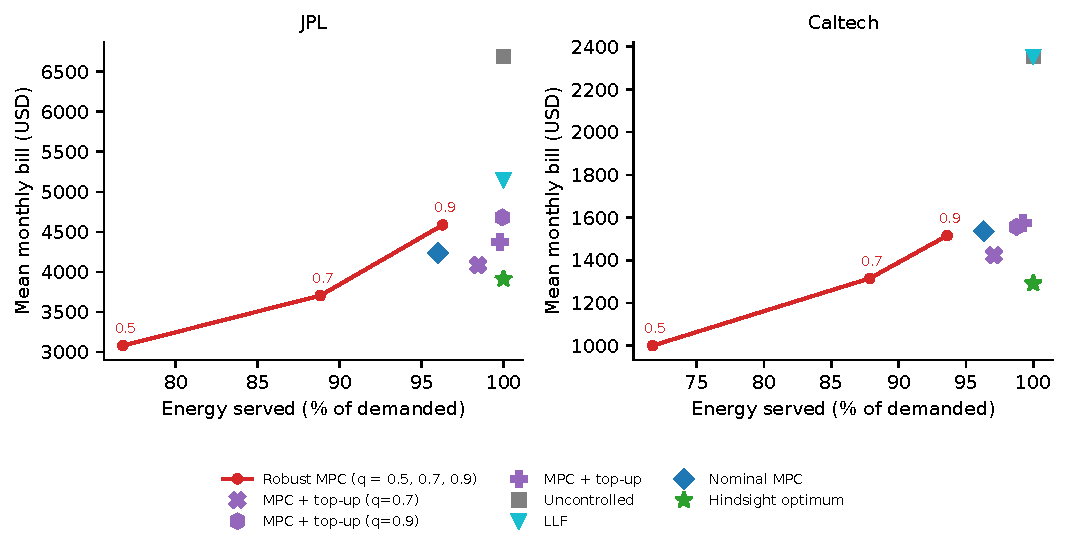
\includegraphics[width=0.7\textwidth]{figures/Fig5_price_of_robustness.pdf}
\caption{Bill against energy served (six-month means). Robust MPC traces a trade-off that stays inside the region reachable by the hindsight optimum; the top-up variants move close to full service.}
\label{fig:frontier}
\end{figure}

\subsection{Peak-state top-up}\label{sec:res:topup}
The top-up rule changes the picture (Table~\ref{tab:main}, Fig.~\ref{fig:frontier}). It is best understood as a more efficient use of electrical capacity: the site has already paid, through the demand charge, for a connection of $\hat P^F$ kilowatts this month, and top-up turns otherwise idle paid-for capacity into delivered EV energy. Applied to nominal MPC, it raises energy served to 99.8\% at JPL and 99.2\% at Caltech, and vehicles fully served to 98.9\% and 96.0\%. The monthly peak and demand charge stay exactly those of nominal MPC. The added cost is the energy price of the extra kWh: 142\,USD per month at JPL for about 800\,kWh, and 39\,USD per month at Caltech for about 210\,kWh, roughly 0.18--0.19\,USD/kWh. The bill remains 35\% (JPL) and 33\% (Caltech) below uncontrolled charging, and 15\% below LLF at JPL. The penalised cost falls to 4,610\,USD at JPL and 1,837\,USD at Caltech, the lowest of all online policies at both sites.

Combining top-up with robust targets gives a tunable operating point. At $q=0.7$ the lower targets keep the peak at 112\,kW (JPL) and 41\,kW (Caltech), and the top-up then serves 98.5\% and 97.1\% of energy. The JPL bill is 4,085\,USD, within 4.3\% of the hindsight optimum on average. At $q=0.9$ with top-up, service at JPL reaches 99.9\% (99.6\% of vehicles), but the higher peak costs 20.9\% over the optimum. Operators can therefore choose between a lower bill and fuller service with one parameter, provided top-up is present; without top-up, the same parameter only trades service for cost.

\subsection{Sensitivity}
Table~S4 of the Supplementary Material reports the sensitivity runs for August and November. Without a demand charge the controllers have no reason to flatten load, and the JPL peak rises to the 195\,kW capacity (Section~\ref{sec:res:tariff}). With twice the demand charge, nominal MPC still serves 96.1\% (JPL) and 95.2\% (Caltech) of energy, whereas robust MPC at $q=0.9$ serves only 91.2\% and 74.2\%, because its earlier deadlines can only be met by raising a peak that costs more than the shortfall penalty. With 30- or 90-day calibration windows, bills and energy served change by less than 1\%, so the negative result is not an artefact of the window length. Raising the shortfall penalty to 20\,USD/kWh leaves service at about 96\%: the shortfall follows from the targets the declarations set, which is why more information or top-up fixes it and re-weighting the objective does not.

\subsection{Tariff design determines whether flexibility is delivered}\label{sec:res:tariff}
Fig.~\ref{fig:tariff} shows how the demand-charge level changes what peak-state control delivers. The sweep uses August and November only (uncontrolled peaks 308 and 116\,kW).
\emph{Without a demand charge, no peak reduction is delivered.} At Caltech the controlled peak equals the uncontrolled peak (116\,kW in August and November). At JPL the only reduction (37\%) is the one the 195\,kW capacity limit imposes on every controlled policy. Without a demand charge, MPC + top-up cannot lower the bill: at JPL it is 1\% more expensive than uncontrolled charging because top-up then fills capacity regardless of price. \emph{A modest demand charge is enough to obtain almost all of the controller's peak reduction.} At 5\,USD/kW-month, about a third of the TOU-EV-4 value, the peak reduction is 55--56\%, essentially the same as at the tariff value (54--56\%) and at twice that value (56--60\%). Beyond this point the demand-charge level mainly scales the monetary saving: 21\% at 5\,USD/kW-month, 37\% at the tariff value and 45--48\% at twice that value. \emph{The online controller's peak saturates while the optimum's does not.} With perfect information the optimum keeps lowering the peak as the demand charge rises, to 68\% reduction at both sites. The online controller's peak is limited by the information available at the time of each decision rather than by the price.
The existence of a demand charge, rather than its exact level, therefore decides whether smart charging delivers local peak reduction. Tariff architecture is thus a precondition for realising the flexibility that controllers can technically provide.





\begin{figure}[!htbp]
\centering
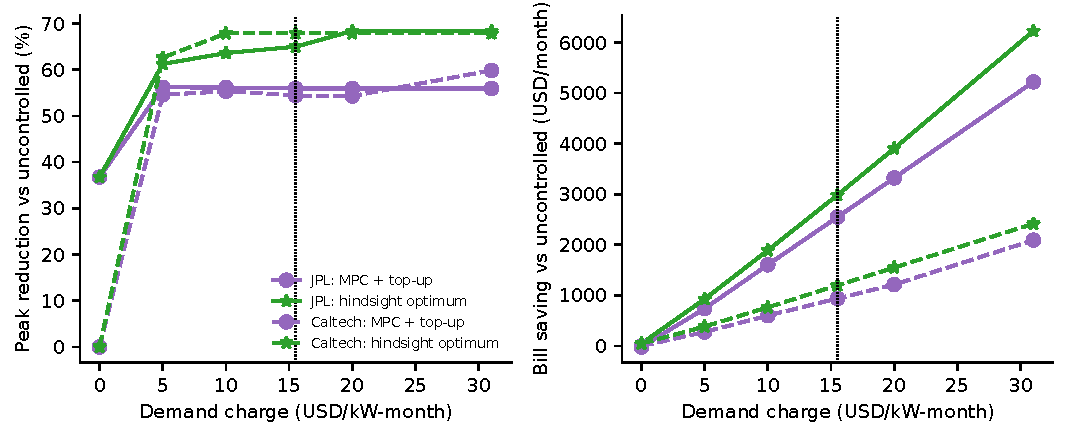
\includegraphics[width=0.7\textwidth]{figures/Fig13_tariff_design.pdf}
\caption{Tariff-design sweep (August and November 2019): peak reduction and monthly bill saving relative to uncontrolled charging as functions of the demand charge. The dotted line marks the TOU-EV-4 value.}
\label{fig:tariff}
\end{figure}

\subsection{Out-of-sample validation on held-out 2021 sessions}\label{sec:res:heldout}
Because top-up was designed after the 2019 diagnosis, we test all policies unchanged on the 2021 extract. Calibration uses the 60 days before each test month (May--June 2021), and the tests cover July and August 2021 (1,605 JPL and 836 Caltech sessions). It is a demanding test: volumes are lower after the pandemic and driver behaviour has shifted: the median claimed driver now leaves 0.4--0.5\,h (JPL) and 1.8--2.0\,h (Caltech) earlier than declared, instead of later, and the median delivered-to-declared energy ratio falls to 0.53--0.54 and 0.40--0.41. Table~\ref{tab:heldout} reports the results.
\emph{The service gap reappears, larger.} Nominal MPC cuts the bill by 30\% (JPL) and 43\% (Caltech) and the peak by 42\% and 53\%, but serves only 91.0\% and 83.7\% of the energy, with 81.7\% and 75.7\% of vehicles fully served. \emph{Top-up replicates.} MPC + top-up raises energy served to 98.6\% (JPL) and 97.1\% (Caltech) and vehicles fully served to 96.3\% and 95.0\%, with exactly the same peaks as nominal MPC. Bills remain 24\% and 34\% below uncontrolled charging. At JPL its penalised cost (3,580\,USD) is the lowest of all online policies and below LLF and uncontrolled charging (3,737\,USD). At Caltech it is the lowest online value but slightly above uncontrolled charging (1,327 against 1,261\,USD), because the remaining 2.9\% shortfall, valued at 5\,USD/kWh, outweighs the bill saving at this small site. \emph{Calibrated robustness fails more severely.} Under the behavioural shift, the $q=0.9$ deadline shifts move 5--8\,h earlier. The resulting targets can only be met by raising the peak, so the controller accepts shortfalls: energy served falls to 56\% (JPL) and 35\% (Caltech), and top-up recovers only part of it. At $q=0.7$ with top-up, JPL still reaches 97.3\% served, but Caltech only 84.2\%.
The held-out test thus confirms both central findings out of sample: top-up retains the peak and bill reductions with near-complete service, and quantile robustness calibrated on declarations is fragile once behaviour drifts.

\begin{table}[!htbp]
\centering
\caption{Out-of-sample validation on held-out 2021 sessions (means over July and August 2021).}
\label{tab:heldout}
\footnotesize
\setlength{\tabcolsep}{1.5pt}
\begin{tabular*}{\textwidth}{@{\extracolsep{\fill}}llrrrrrr@{}}
\hline
Site & Policy & \makecell[c]{Bill\\(USD)} & \makecell[c]{Saving vs\\unc. (\%)} & \makecell[c]{Peak\\(kW)} & \makecell[c]{Served\\(\%)} & \makecell[c]{EVs\\full (\%)} & \makecell[c]{Penalised\\(USD)} \\
\hline
JPL & Uncontrolled & 3,737 & +0.0 & 151.0 & 100.0 & 100.0 & 3,737 \\
JPL & LLF & 3,737 & +0.0 & 151.0 & 100.0 & 100.0 & 3,737 \\
JPL & Nominal MPC & 2,614 & +30.0 & 87.4 & 91.0 & 81.7 & 7,078 \\
JPL & Robust MPC, $q$=0.7 & 2,423 & +34.9 & 79.3 & 85.2 & 63.9 & 9,893 \\
JPL & Robust MPC, $q$=0.9 & 1,459 & +61.1 & 36.3 & 55.8 & 40.3 & 24,099 \\
JPL & MPC + top-up & 2,822 & +24.4 & 87.4 & 98.6 & 96.3 & 3,580 \\
JPL & MPC + top-up, $q$=0.7 & 2,705 & +27.4 & 79.2 & 97.3 & 92.7 & 4,167 \\
JPL & MPC + top-up, $q$=0.9 & 1,580 & +58.0 & 36.3 & 62.4 & 51.1 & 20,834 \\
JPL & Hindsight opt. & 2,468 & +34.5 & 63.7 & 100.0 & 100.0 & 2,468 \\
\hline
Caltech & Uncontrolled & 1,261 & +0.0 & 52.7 & 100.0 & 100.0 & 1,261 \\
Caltech & LLF & 1,261 & +0.0 & 52.7 & 100.0 & 100.0 & 1,261 \\
Caltech & Nominal MPC & 723 & +42.5 & 24.9 & 83.7 & 75.7 & 3,402 \\
Caltech & Robust MPC, $q$=0.7 & 521 & +58.2 & 13.6 & 68.9 & 54.9 & 5,786 \\
Caltech & Robust MPC, $q$=0.9 & 262 & +79.2 & 6.9 & 35.4 & 28.2 & 10,932 \\
Caltech & MPC + top-up & 827 & +34.1 & 24.9 & 97.1 & 95.0 & 1,327 \\
Caltech & MPC + top-up, $q$=0.7 & 601 & +51.8 & 13.3 & 84.2 & 80.7 & 3,328 \\
Caltech & MPC + top-up, $q$=0.9 & 349 & +72.4 & 6.9 & 52.3 & 47.4 & 8,223 \\
Caltech & Hindsight opt. & 776 & +38.5 & 22.1 & 99.9 & 99.3 & 798 \\
\hline
\end{tabular*}
\par\smallskip\parbox{\textwidth}{\scriptsize Calibration uses the 60 days before each test month. EDF coincides with LLF and is omitted.}
\end{table}


\subsection{Robustness of the top-up rule}\label{sec:res:topuprob}
Because the top-up rule was designed after the 2019 diagnosis, we also test it, unchanged, under conditions it was not designed for: a site capacity cut to 75\% and 50\% of its value, twice the demand charge, 30- and 90-day calibration windows, and a shortfall penalty of 20\,USD/kWh (four times the base value). Each scenario is run on August and November 2019 and on the held-out July and August 2021 (Table~S5 of the Supplementary Material).
The service gain persists in every scenario: top-up raises energy served from 94.1--96.5\% to 97.1--99.8\% in 2019 and from 83.0--91.5\% to 95.6--98.7\% in 2021, a gain of 2.4--3.7 and 7.2--13.5 percentage points. It never raises the peak: across all 56 scenario--site--month runs, the MPC + top-up peak equals the nominal MPC peak, except in one month where it is 1.8\,kW lower because energy delivered early reduced later needs. The weakest cases are those where capacity or cost binds. With JPL's capacity halved to 97.5\,kW, the limit binds below the nominal peak and top-up serves 97.1\% in 2019, with 90.9\% of vehicles fully served. With twice the demand charge, Caltech reaches 97.6\% (2019) and 95.6\% (2021), because the controller holds a lower peak and leaves less headroom to fill. These tests, like the held-out evaluation, are simulations on recorded sessions. They show that the rule's benefit does not depend on the particular settings under which it was devised; they do not show how drivers would respond to it in operation, which only a field trial can establish. Because service is measured against historically delivered energy, which the ACN's own controller may have truncated, we also raise every session's need to 1.1 and 1.25 times its recorded energy, capped at what its estimated maximum rate can deliver while plugged in, leaving declarations unchanged (Table~S6). Total demand then rises by 8--10\% and 18--23\%. Nominal MPC falls to 81--95\% served, whereas MPC + top-up still serves 96.0--99.5\%, never with a higher peak than nominal MPC, and with peak reductions of 43--61\%; the hindsight optimum serves at least 99.7\%. The larger the unrecorded demand, the larger the gain from top-up, because the extra energy is exactly what declarations do not request.


\subsection{PV-aware control: from coincidence to self-consumption}\label{sec:res:pvaware}
Table~\ref{tab:pv} reports the PV scenario of Section~\ref{sec:pvaware}. Its figures are scenario estimates under clear-sky irradiance with a horizontal, energy-neutral array, not verified performance under measured solar conditions. With an energy-neutral PV array behind the meter, uncontrolled charging still sets an import peak of 282\,kW at JPL and 79\,kW at Caltech, because the morning arrival spike precedes most of the solar output.
\emph{At JPL, PV awareness adds a large second layer of flexibility.} PV-unaware MPC + top-up lowers the import peak to 128\,kW. Making the controller PV-aware lowers it further to 73\,kW, 26\% of the uncontrolled value. The bill falls by another 32\% (from 2,777 to 1,878\,USD), PV self-sufficiency rises from 50.7\% to 58.0\%, and 99.2\% of energy is still served. With moderate robustness ($q=0.7$) the import peak reaches 46\,kW and self-sufficiency 64.4\%, close to the PV-aware optimum (43\,kW; 66.5\%), at 97.0\% energy served. \emph{At Caltech, PV awareness alone adds nothing.} The PV-aware and PV-unaware top-up controllers give almost the same import peak (26 and 25\,kW) and self-sufficiency (about 60\%), because Caltech's later arrivals already coincide with solar output. Only the robust variant moves further (16\,kW; 63.6\%), and the optimum shows that 72.7\% self-sufficiency would be attainable with perfect information.
The value of renewable-aware control is therefore site-specific. It is largest where arrivals precede solar output. As with the demand charge, the gap to the optimum is limited by the information drivers provide rather than by the solar resource.

\begin{table}[!htbp]
\centering
\caption{PV-aware control with an energy-neutral clear-sky PV array (means over July--December 2019; all policies billed on grid import).}
\label{tab:pv}
\footnotesize
\setlength{\tabcolsep}{1.5pt}
\begin{tabular*}{\textwidth}{@{\extracolsep{\fill}}llrrrrrr@{}}
\hline
Site & Policy & \makecell[c]{Bill\\(USD)} & \makecell[c]{Import\\peak (kW)} & \makecell[c]{Served\\(\%)} & \makecell[c]{EVs\\full (\%)} & \makecell[c]{PV self-\\suff. (\%)} & \makecell[c]{Penalised\\(USD)} \\
\hline
JPL & Uncontrolled & 5,190 & 281.9\,{\scriptsize(264--297)} & 100.0 & 100.0 & 46.7 & 5,190 \\
JPL & Top-up, PV-unaware & 2,777 & 127.6\,{\scriptsize(121--135)} & 99.9 & 99.5 & 50.7 & 2,876 \\
JPL & PV-aware top-up & 1,878 & 73.3\,{\scriptsize(57--94)} & 99.2 & 97.3 & 58.0 & 2,692 \\
JPL & PV-aware, $q$=0.7 & 1,447 & 46.2\,{\scriptsize(34--57)} & 97.0 & 91.2 & 64.4 & 4,626 \\
JPL & PV-aware opt. & 1,311 & 43.3\,{\scriptsize(38--47)} & 100.0 & 99.9 & 66.5 & 1,323 \\
\hline
Caltech & Uncontrolled & 1,487 & 79.3\,{\scriptsize(65--91)} & 100.0 & 100.0 & 56.1 & 1,487 \\
Caltech & Top-up, PV-unaware & 642 & 25.0\,{\scriptsize(19--31)} & 99.2 & 97.1 & 60.5 & 922 \\
Caltech & PV-aware top-up & 666 & 26.2\,{\scriptsize(21--35)} & 99.3 & 96.8 & 60.2 & 921 \\
Caltech & PV-aware, $q$=0.7 & 492 & 16.3\,{\scriptsize(15--21)} & 97.4 & 91.9 & 63.6 & 1,401 \\
Caltech & PV-aware opt. & 401 & 15.5\,{\scriptsize(12--21)} & 100.0 & 99.9 & 72.7 & 407 \\
\hline
\end{tabular*}
\par\smallskip\parbox{\textwidth}{\scriptsize Monthly range of the import peak below the mean. PV self-sufficiency is the share of delivered EV energy supplied by PV. Surplus PV is curtailed without export credit.}
\end{table}


\subsection{Transformer hosting limits: deliverable flexibility}\label{sec:res:xfmr}
Table~\ref{tab:xfmr} reports the transformer scenarios of Section~\ref{sec:xfmr}.
\emph{Uncontrolled charging overloads.} On a transformer rated at 50\% of its uncontrolled peak, uncontrolled charging reaches 2.1 (JPL) and 2.2 (Caltech) times the rating, for 38 and 32 hours per month. At a 35\% rating the loading reaches about 3 per unit for 54--57 hours per month, with 4,427\,kWh (JPL) and 1,141\,kWh (Caltech) of monthly energy above the rating. \emph{Within a 50\% rating, controlled charging delivers almost full service.} MPC + top-up stays at 0.92 (JPL) and 0.98 (Caltech) of the rating while serving 99.8\% and 99.0\% of energy, so its demand-charge-driven peak reduction already satisfies the network limit with headroom. \emph{At a 35\% rating, the limit binds for every online policy.} MPC + top-up then serves 98.4\% (JPL) and 96.6\% (Caltech) of energy, and LLF serves 98.3\% and 97.2\%. The hindsight optimum still serves 100\% and 99.7\% within the same rating. The limit is therefore physically compatible with full service; online controllers fall short because they lack information, not capacity. Under a tight network limit the simple LLF rule is as good as MPC on service, because the binding constraint is capacity rather than cost.
For a distribution operator, these results translate site-level control into a deliverable quantity. A workplace fleet that would load its transformer to two or three times its rating can be held within the rating, with only 0--3\% of energy unserved, by controllers that need nothing beyond plug-in events and meter readings. These are statements about a static import limit at the connection point. They show that the required energy fits under the rating, not that the transformer stays within its thermal limits, that feeder voltages remain in range or that phases stay balanced; Section~\ref{sec:discussion} returns to these limitations.

\begin{table}[!htbp]
\centering
\caption{Transformer hosting scenarios (means over August and November 2019).}
\label{tab:xfmr}
\footnotesize
\setlength{\tabcolsep}{1.5pt}
\begin{tabular*}{\textwidth}{@{\extracolsep{\fill}}lllrrrrr@{}}
\hline
Site & \makecell[c]{Rating\\kW (\%)} & Policy & \makecell[c]{Max loading\\(p.u.)} & \makecell[c]{Overload\\(h/mo)} & \makecell[c]{Overload\\(kWh/mo)} & \makecell[c]{Served\\(\%)} & \makecell[c]{EVs\\full (\%)} \\
\hline
JPL & 148 (50\%) & Uncontrolled & 2.08 & 37.8 & 2,342 & 100.0 & 100.0 \\
JPL & 148 (50\%) & LLF & 1.00 & 0.0 & 0 & 99.9 & 99.4 \\
JPL & 148 (50\%) & Top-up & 0.92 & 0.0 & 0 & 99.8 & 98.7 \\
JPL & 148 (50\%) & Top-up, $q$=0.7 & 0.74 & 0.0 & 0 & 98.6 & 94.3 \\
JPL & 148 (50\%) & Hindsight opt. & 0.73 & 0.0 & 0 & 100.0 & 100.0 \\
JPL & 104 (35\%) & Uncontrolled & 2.98 & 57.2 & 4,427 & 100.0 & 100.0 \\
JPL & 104 (35\%) & LLF & 1.00 & 0.0 & 0 & 98.3 & 95.4 \\
JPL & 104 (35\%) & Top-up & 1.00 & 0.0 & 0 & 98.4 & 93.8 \\
JPL & 104 (35\%) & Top-up, $q$=0.7 & 1.00 & 0.0 & 0 & 97.9 & 91.9 \\
JPL & 104 (35\%) & Hindsight opt. & 0.98 & 0.0 & 0 & 100.0 & 100.0 \\
\hline
Caltech & 52 (50\%) & Uncontrolled & 2.21 & 31.7 & 498 & 100.0 & 100.0 \\
Caltech & 52 (50\%) & LLF & 1.00 & 0.0 & 0 & 99.7 & 98.3 \\
Caltech & 52 (50\%) & Top-up & 0.98 & 0.0 & 0 & 99.0 & 95.4 \\
Caltech & 52 (50\%) & Top-up, $q$=0.7 & 0.81 & 0.0 & 0 & 96.7 & 89.8 \\
Caltech & 52 (50\%) & Hindsight opt. & 0.71 & 0.0 & 0 & 100.0 & 100.0 \\
Caltech & 37 (35\%) & Uncontrolled & 3.16 & 54.2 & 1,141 & 100.0 & 100.0 \\
Caltech & 37 (35\%) & LLF & 1.00 & 0.0 & 0 & 97.2 & 92.6 \\
Caltech & 37 (35\%) & Top-up & 1.00 & 0.0 & 0 & 96.6 & 90.1 \\
Caltech & 37 (35\%) & Top-up, $q$=0.7 & 1.00 & 0.0 & 0 & 95.5 & 87.9 \\
Caltech & 37 (35\%) & Hindsight opt. & 0.96 & 0.0 & 0 & 99.7 & 99.7 \\
\hline
\end{tabular*}
\par\smallskip\parbox{\textwidth}{\scriptsize Ratings are 50\% and 35\% of the six-month mean uncontrolled peak. Controlled policies treat the rating as a hard limit; uncontrolled charging does not.}
\end{table}




\subsection{Tariff archetypes}\label{sec:res:arch}
Under both stylised archetypes, which keep the demand charge (Table~S7 of the Supplementary Material), MPC + top-up reduces the peak by the same 56\% (JPL) and 54\% (Caltech) as under TOU-EV-4, with 99.8\% and 99.0\% of energy served: the demand charge, not the energy-price structure, drives peak reduction. The energy-price conflict disappears. Flattening raises the energy cost by 6.1\% (JPL) and 5.4\% (Caltech) under TOU-EV-4, but by only 2.6\% and $-0.7$\% under the evening-peak archetype and by $-0.2$\% and $-0.9$\% under a flat price, so the total bill saving rises from 37\% to 40--41\%. Tariffs that combine a demand charge with an evening peak or a flat energy price, as is common outside California, therefore reward both local peak reduction and midday solar absorption.

%======================================================================
\section{Discussion}\label{sec:discussion}
%======================================================================
\subsection{From technical to grid-usable flexibility}
The technical flexibility of workplace charging, bounded by parking duration and connected capacity, differs from the grid-usable flexibility that a controller can deliver while keeping drivers served and that a network operator can rely on. This requires evaluating charging service, operator cost and grid flexibility at the connection point jointly. Uncontrolled charging maximises service and minimises flexibility; robust MPC at low $q$ looks best on cost and peak alone precisely because it withholds energy, so assessments that report only one or two dimensions can rank policies wrongly. Service is measured here against the energy each vehicle received in 2019 under the ACN's own control, so a figure such as 99\% served means that the controllers reproduce the recorded energy deliveries, not that they meet every driver's unconstrained need; where the recorded deliveries were themselves truncated, true service would be lower for all policies alike. MPC + top-up is the only online policy that is close to the frontier on all three at once, and combining it with moderate robustness moves further along the flexibility axis at a small service cost.

\subsection{Information quality, not optimisation, limits realisable flexibility}
The negative result on calibrated robustness is an empirical energy-management finding, not a failure of the optimisation method: better mathematical protection cannot compensate for structurally poor information. Declared energy is an upper bound for most drivers and a lower bound for a few, and declared departure is late for about a third. Constraint-wise robust counterparts over boxes, whether built from quantiles as here or from more elaborate data-driven sets \cite{Bertsimas2018DataDriven,Esfahani2018Wasserstein}, can shift and scale targets but cannot add energy that no target requests, and they pay for early-leaver protection with higher peaks. What works is recourse to realised information: the observation that a vehicle is still drawing current, used by top-up. This is consistent with the caution against over-conservative robust solutions \cite{Bertsimas2004Price,Gorissen2015Guide}. It also suggests that per-driver prediction \cite{Lee2019ACNData,Wang2016Predictive,Kreft2024Predictability} and incentives for accurate declarations are the most promising levers for realising more of the flexibility that parking durations imply.

\subsection{Implications for energy-system actors}
\emph{Charging-site operators} gain roughly a third of the electricity bill and half of the site peak from demand-charge-aware control; greedy capacity-constrained rules capture peak reduction only where capacity binds. Headroom below the month's realised peak should be filled with top-up, which costs only the energy price, and energy served should always be reported alongside savings.
\emph{Aggregators and utilities} can treat the realised month-to-date peak $\hat P^F(\tau)$, set early in the billing month and then defended, as a verifiable firm-capacity limit offered to a distribution operator, aggregator or virtual power plant; the formulation extends to this by replacing the site peak with a contracted import limit or network signal. A controlled workplace fleet can be expected to deliver about half of its uncontrolled peak as firm reduction, enough to keep a half-rated transformer within its rating; in the clear-sky PV scenario, PV-aware control at a site like JPL lowers the import peak to about a quarter. Deeper reductions, up to the 63--68\% achieved in hindsight, need better information than declarations.
\emph{Tariff designers} should note that the presence of a demand charge, not its level, decides whether local peak reduction is delivered. Commercial EV rates that suspend demand charges \cite{CPUCEVRates} remove the incentive to flatten workplace load, whereas a small demand charge, or an equivalent subscription or import-limit product, unlocks it. Moving the on-peak energy window to the evening, or using a flat energy price, removes the conflict with midday charging.

\subsection{Deployment, network constraints and generalisability}
In real time, the controller needs plug-in events, declarations where available, a per-port signal showing whether a vehicle still draws current, the site meter reading and the tariff, all available in networked systems of the ACN type \cite{Lee2021ACN}. Each re-solve is a sparse LP that grows linearly with the connected vehicles and the horizon: mean solve times were 0.013\,s for JPL's 52 ports and 0.005\,s at Caltech on one core, and the monthly hindsight LP took 8.1\,s and 2.3\,s. Sites with hundreds of ports remain well within minute-scale control loops; top-up is a sorting step, and calibration needs only a rolling store of past sessions.

The transformer analysis is a static import limit. It does not model transformer thermal dynamics or ageing, feeder voltage, three-phase imbalance or power flow, all present in real installations \cite{Lee2021ACN,Lee2021ACNSim} and distribution networks \cite{ClementNyns2010,deHoog2015Network,Gong2012Transformer}. The peak-state structure is compatible with richer models: per-phase or per-transformer constraints can be added to the LP \cite{Lee2021ACN,deHoog2015Network}, transformer or feeder peaks can be tracked as additional peak states, and top-up then fills headroom below the tightest limit.

Three elements of the findings are structural and should transfer: the monthly peak-state logic, under which capacity paid for early in the month is free thereafter; the gap between declared and realised behaviour, documented in other datasets \cite{Kreft2024Predictability,Flammini2019Stats}; and the re-use of paid-for capacity through top-up. The TOU-EV-4 price windows, the commuting patterns of two southern Californian campuses, Level-2 charger power, site capacities and the 2019 period are context-specific, so the magnitudes reported here should be re-estimated elsewhere. The ordering of policies and the mechanism behind the robustness failure are expected to hold wherever declarations are biased and wide, as the held-out 2021 test and the tariff archetypes indicate.

\subsection{Limitations}
Vehicles are ideal loads that accept energy at up to $\bar r_i$ until full, without battery tapering, and $\bar r_i$ is estimated because the extract lacks the done-charging time. The energy delivered by the ACN is used as each vehicle's demand and may have been truncated by the controller in place at the time, so service figures measure delivery relative to historical charging, not necessarily drivers' actual needs; the higher-demand sensitivity (Section~\ref{sec:res:topuprob}) bounds, but does not remove, this uncertainty. The PV scenarios use clear-sky irradiance and a horizontal array, because measured irradiance for the sites was not accessible to us; they overstate solar output on cloudy days, and surplus PV is curtailed without export credit. Transformer limits are static, holidays and customer charges are omitted, and the study covers two sites, six test months and a two-month held-out period. The top-up rule was designed after the 2019 diagnosis and validated in simulation on two held-out 2021 months and under altered capacity, tariff, calibration and penalty settings; it has not been tested in a field deployment, where drivers might respond to the fuller service it offers.

%======================================================================
\section{Conclusions}\label{sec:conclusion}
%======================================================================
The flexibility of workplace EV charging is not determined only by how long cars are parked or how much charging capacity is connected. On 13,623 real sessions from two California workplaces, peak-state control that prices only increments above the month-to-date peak roughly halved the site peak (from 296 to 140\,kW and from 105 to 52\,kW). Acting on driver declarations, however, left about one vehicle in eight short of its energy, and robust counterparts calibrated to empirical declaration errors did not close this gap. Re-using capacity already billed in the month restored service to above 99\% of the historically delivered energy without a new peak; on held-out 2021 sessions, and under altered capacity, tariff and calibration settings, it again raised service to 96--99\% without raising the peak. These are simulation results on recorded sessions, not field results.

The same controllers held a transformer rated at half the uncontrolled peak within its rating with near-complete service, where uncontrolled charging overloaded it by a factor of two. In a clear-sky PV scenario, where arrivals precede solar output, PV-aware control lowered the import peak to about a quarter of its uncontrolled value. The presence of a demand charge, not its level or the energy-price structure, decided whether any peak reduction was delivered.

Information quality and tariff design therefore jointly determine how much of the technical flexibility of workplace charging can be realised without degrading mobility service. Future work should test the controllers in the field, over longer periods and at other sites; replace population-level uncertainty sets with per-driver predictions and declaration incentives; add transformer thermal, voltage and three-phase models as further peak states; and test the realised peak as a contracted flexibility product for aggregators and virtual power plants.
